\documentclass[a4paper]{article}

\usepackage[utf8]{inputenc}
\usepackage{parskip}
\usepackage[margin=1in]{geometry}
\usepackage{graphicx}
\usepackage{todonotes}
\usepackage{hyperref}

\widowpenalty=10000

\title{SudokuMP User Manual, RPC Version}
\author{Johan Kütt, A32401}
\date{January 2, 2018}

\begin{document}
\maketitle

\section{Installation}

The application is available from \url{https://github.com/johankytt/SudokuMP/tree/rpc\_p2p}. No special installation procedures are required by the application itself.

The following libraries are required to run the application:
\begin{itemize}
	\item[--] The graphical user interface relies on the PySide library which is freely available both from the web and from package managers. Version 1.2.2 of the library was used for development.
	\item[--] RPC over message queue is implemented using SnakeMQ. The version of the library included with the application should be used as the one available on the web contains a critical bug that renders the library non-functional under certain conditions.
\end{itemize}

The logging output shown on the command line is controlled by adjusting \texttt{level=logging.XXX} in \texttt{common/smp\_common.py}. Setting it below INFO for normal use is not recommended as the console will be flooded with large amounts of messages.


% ================================

\section{Running the Server}

The server is a purely command line application. It is started by running the script "start\_server.py". The only configurable options are it's listening address and port, which are set as shown in its command line help (also shown below). If the host argument is not given, the public address of the default network interface is used. The server process can be stopped by issuing Ctrl-C on the command line.

\textbf{Note:} The SnakeMQ based indirect messaging system is built into the server and loaded automatically.

\hrulefill

\texttt{usage: start\_server.py [-h] [-H HOST] [-P PORT]\\
~\\
SudokuMP Server\\
~\\
optional arguments:\\
-h, --help            show this help message and exit\\
-H HOST, --host HOST  IP or Name of the host server (default:\ 192.168.1.65)\\
-P PORT, --port PORT  Listening port of the host server (default:\ 22122)
}

\hrulefill

% ===============================

\section{Running the Client Application}

The client application is run similarily to the server from the command line by executing \texttt{python start\_client.py}. The client takes no command line arguments.

On opening the application the lobby window will be shown. On the right hand side are the user controls and on the left the server game list which will be populated once a connection is made.

Before a connection is established most controls are disabled to avoid inadvertent clicking.


\subsection{Connecting to the server}

To be able to connect to a server, the user must fill out the player name, server address and server port fields. Once that is done the "Connect" button will be enabled and the user can proceed with establishing the connection.

\textbf{Note:} In this version of the application, automatic server discovery is automatically started on application startup. When a server is found, the server address and port fields are automatically updated with the correct values.

\subsection{Joining a game}

Once the connection is established the server game list will be automatically populated with all games currently available on the server. Note, from here on to obtain latest information the list has to be manually refreshed by clicking the corresponding button.

The desired game should be selected from the list and it will be joined by clicking the "Join Game" button.


\subsection{Creating a new game}

To create a new game, the desired number of players must be entered on the bottom right of the window and the "Create Game" button clicked.


\subsection{Playing the game}

On game join or creation the game window will be shown. On the left hand side is the Sudoku board and on the right game info, including running game duration, player scores and notifications. Clicking the "Leave Game" button on the bottom right will remove the player from the game and take him back to the lobby screen.

Initially the game board will be empty while waiting for other players. Once all required players have joined, the game board will be populated with the initial state and the simultaneous solving of the puzzle can begin.

Number entry mode is entered as usual in tabular applicatons by double clicking, tabbing or hitting enter.

% ===============================

\section{Network Architecture}

Figures \ref{fig:networkArchitecture} and \ref{fig:networkLayout} show the application network architecture and layout.

Automatic server discovery is implemented using UDP broadcast messages and responses. When started, the client periodically sends out a structured broadcast message. When the server, that is listening for broadcast messages, receives and verifies the message it responds directly to the client with its game communication public address.

The game network protocol is implemented using RPC over the SnakeMQ indirect messaging API. The client initially connects to a public connection handling port of the server and is then redirected to a private port belonging to a specific client handler. Both connections use RPC over SnakeMQ.

\textbf{Note:} This network module utilizing SnakeMQ and RPC is a direct port of the previous socket-based implementation. Therefore it may not be the most efficient use of RPC. At the same time the easy portability demonstrates the benefits of the application's modular design.

\textbf{Note:} As the main goal of multiplayer Sudoku is to be concurrent, time uncoupling is in no way a reasonable requirement for the networking solution.

\vfill

\begin{figure}[hb] \centering
	{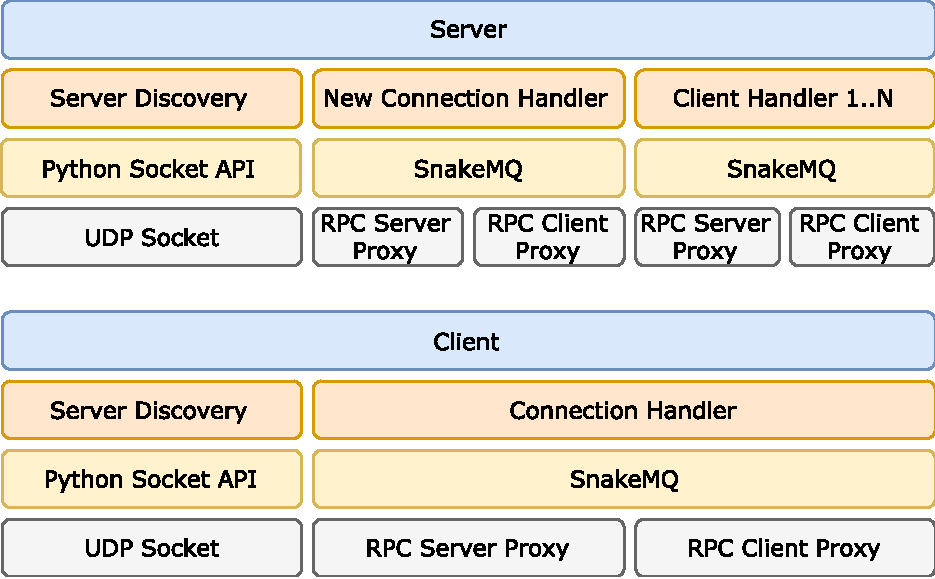
\includegraphics[width=0.87\linewidth]{SMP_Network_Architecture}}
	\caption{SudokuMP Network Architecture}
	\label{fig:networkArchitecture}
\end{figure}

\vfill

\begin{figure}[htb] \centering
	{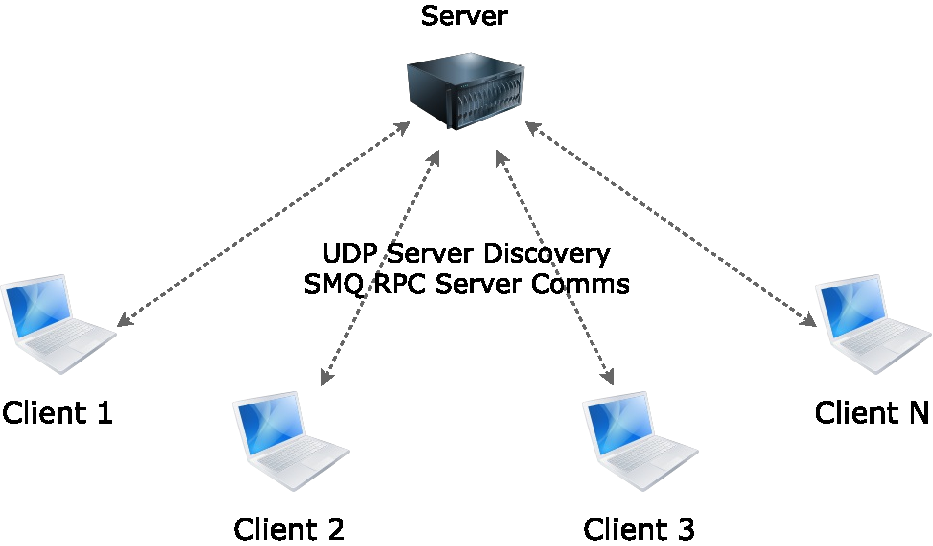
\includegraphics[width=0.87\linewidth]{SMP_Network_Layout}}
	\caption{SudokuMP Network Layout}
	\label{fig:networkLayout}
\end{figure}

\end{document}